%!TeX root = BasiDiDati.tex

\chapter{Ottimizzazione di interrogazioni}
Ogni interrogazione sottomessa al DBMS viene espressa in un linguaggio dichiarativo (es. SQL).\\[0.2ex]
E' necessario, quindi, trovare un'equivalente espressione procedurale (es. algebra relazionale) per generare un piano di esecuzione.\\[0.2ex]
L'espressione algebrica va ottimizzata rispetto alle caratteristche del DBMS a livello fisico e dalla base di dati corrente.

\smallskip
Le fasi di ottimizzazione di una query conistono in:
\begin{enumerate}[itemsep=\smallskipamount]
    \item \textbf{analisi lessicale e sintattica}: verifica che la query sia scritta correttamente
    \item \textbf{ottimizzazione algebrica}: si basa sulle regole dell'algebra relazionale
    \begin{itemize}[label=$\circ$, itemsep=\smallskipamount]
        \item anticipo delle selezioni
        \item anticipo delle proiezioni
    \end{itemize}
    \item \textbf{ottimizzaione dipendente dai metodi di accesso}: si basa sulle statistiche e sulle strutture fisiche (profili delle tabelle)
    \item \textbf{generazione del codice}: si genera un piano di esecuzione per ottenere il risultato della query
\end{enumerate}

\begin{figure}[H]
    \centering
    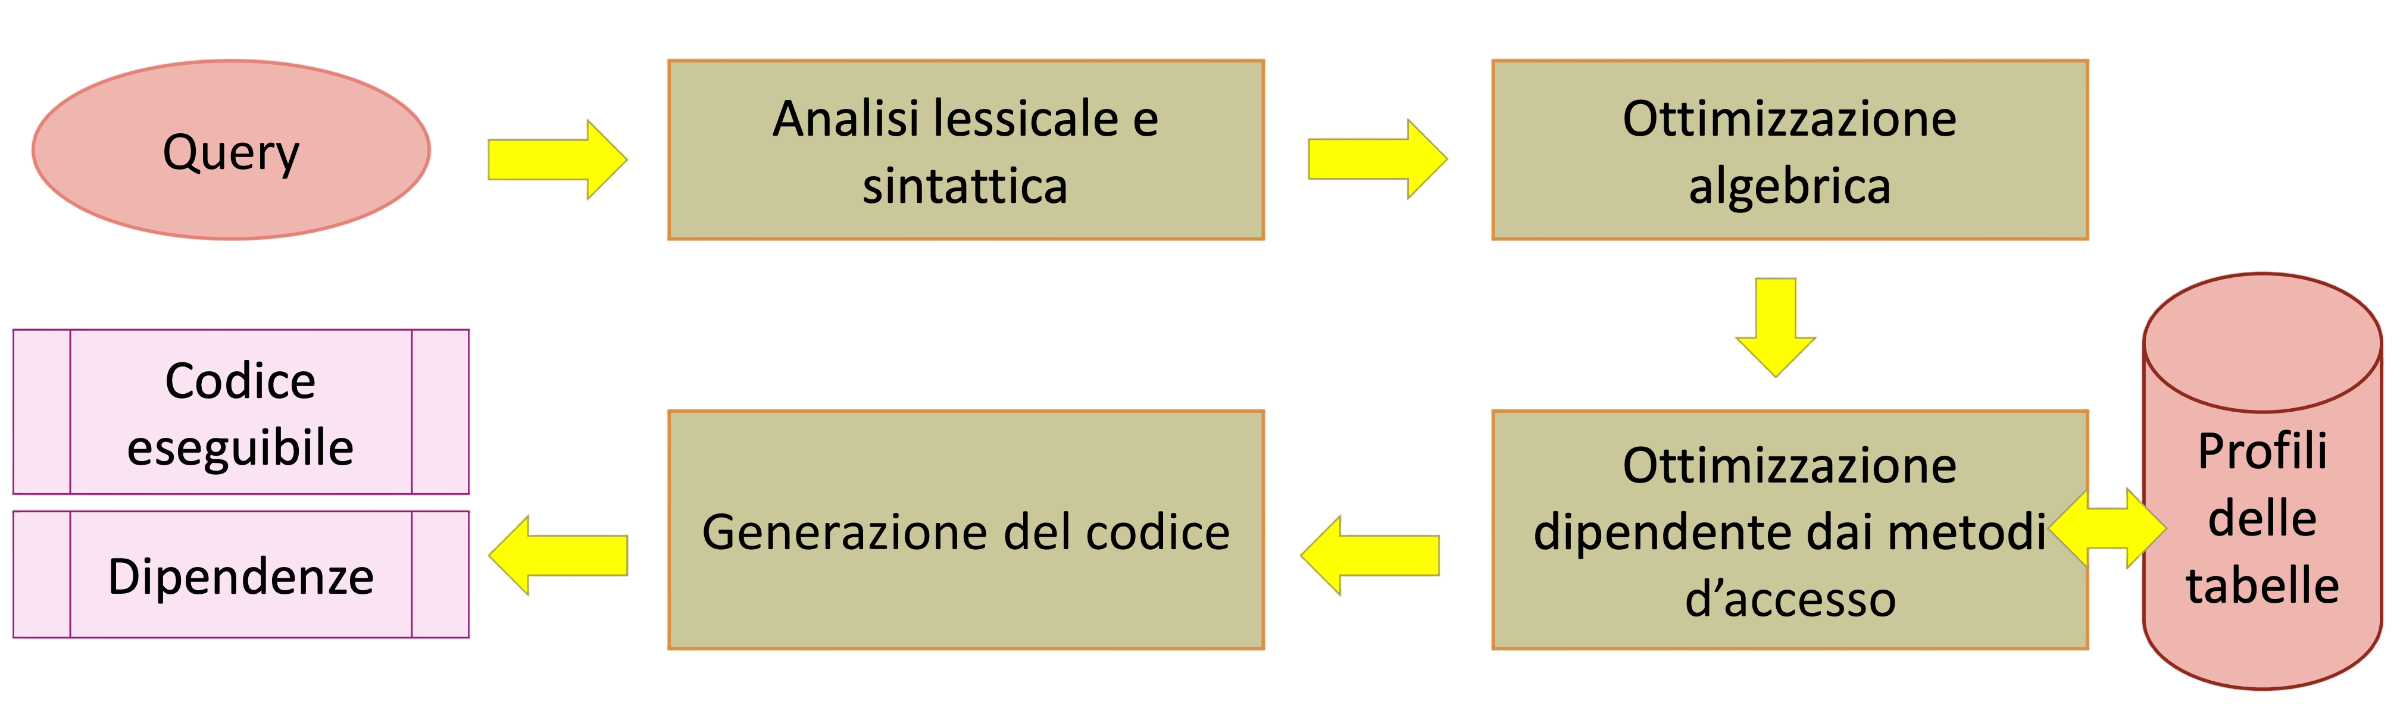
\includegraphics[width=0.75\textwidth]{images/ottimizzazione-query.png}
    \caption{processo di ottimizzazione di una query}
\end{figure}

\section{Ottimizzazione dipendente dai metodi di accesso}
Le operazioni tipiche di accesso supportate dal DBMS sono:
\begin{itemize}[label=$\triangleright$, itemsep=\smallskipamount]
    \item \textbf{scansione delle tuple di una tabella}
    \item \textbf{ordinamento delle tuple}
    \item \textbf{accesso diretto tramite indice}
    \item \textbf{join con diverse implementazioni}
\end{itemize}

\subsection{Scansione sequenziale}
L'operazione di scansione opera contestualmente altre operazioni:
\begin{itemize}[label=$\diamond$, itemsep=\smallskipamount]
    \item \textbf{scansione} + \textbf{proiezione} (senza eliminazione dei duplicati)
    \item \textbf{scansione} + \textbf{selezione} (rispetto a un predicato semplice)
    \item \textbf{scansione} + \textbf{inserimento/cancellazione/modifica}
\end{itemize}

\begin{itemize}[label=$\Rightarrow$, itemsep=\smallskipamount]
    \item \textcolor{red}{\textbf{costo scansione sequenziale}}: $\mathbf{NP(R)}$ (numero di pagine della relazione $\mathrm{R}$)
\end{itemize}

\subsection{Ordinamento}
L'ordinamento viene utilizzato per:
\begin{itemize}[label=$\diamond$, itemsep=\smallskipamount]
    \item \textbf{ordinare il risultato di un'interrogazione} (clausola \texttt{ORDER BY})
    \item \textbf{eliminare duplicati} (clausola \texttt{SELECT DISTINCT})
    \item \textbf{raggruppare tuple} (clausola \texttt{GROUP BY})
\end{itemize}

L'ordinamento viene eseguito su memoria secondaria utilizzando l'algoritmo \textbf{Z-way-Sort-Merge}:
\begin{enumerate}[itemsep=\smallskipamount]
    \item \textbf{sort interno}:
    \begin{enumerate}[itemsep=\smallskipamount]
        \item si leggono una alla volta le pagine della tabella
        \item le tuple di ogni pagina vengono ordinate con un algoritmo di sort interno (es. quick-sort)
        \item ogni pagina ordinata (run) viene scritta su memoria secondaria in un file temporaneo 
    \end{enumerate}
    \item \textbf{merge}: vengono unite le run in un'unica run
\end{enumerate}

\esempio{algoritmo Z-way-Sort-merge}{
    Supponiamo di dover ordinare un input che consiste in una tabella di $\mathrm{NP}$ pagine e di avere a disposizione sono $\mathrm{NB}$ buffer in memoria centrale ($\mathrm{NB < NP}$).

    Per semplicità, consideriamo il caso base a due vie ($\mathrm{Z} = 2$) e supponiamo di avere solo 3 buffer in memoria centrale ($\mathrm{NB} = 3$).

    \smallskip
    Si hanno 4 pagine composte da 3 tuple ciascuna e si vuole ordinare in base alla prima colonna:
    \begin{figure}[H]
        \centering
        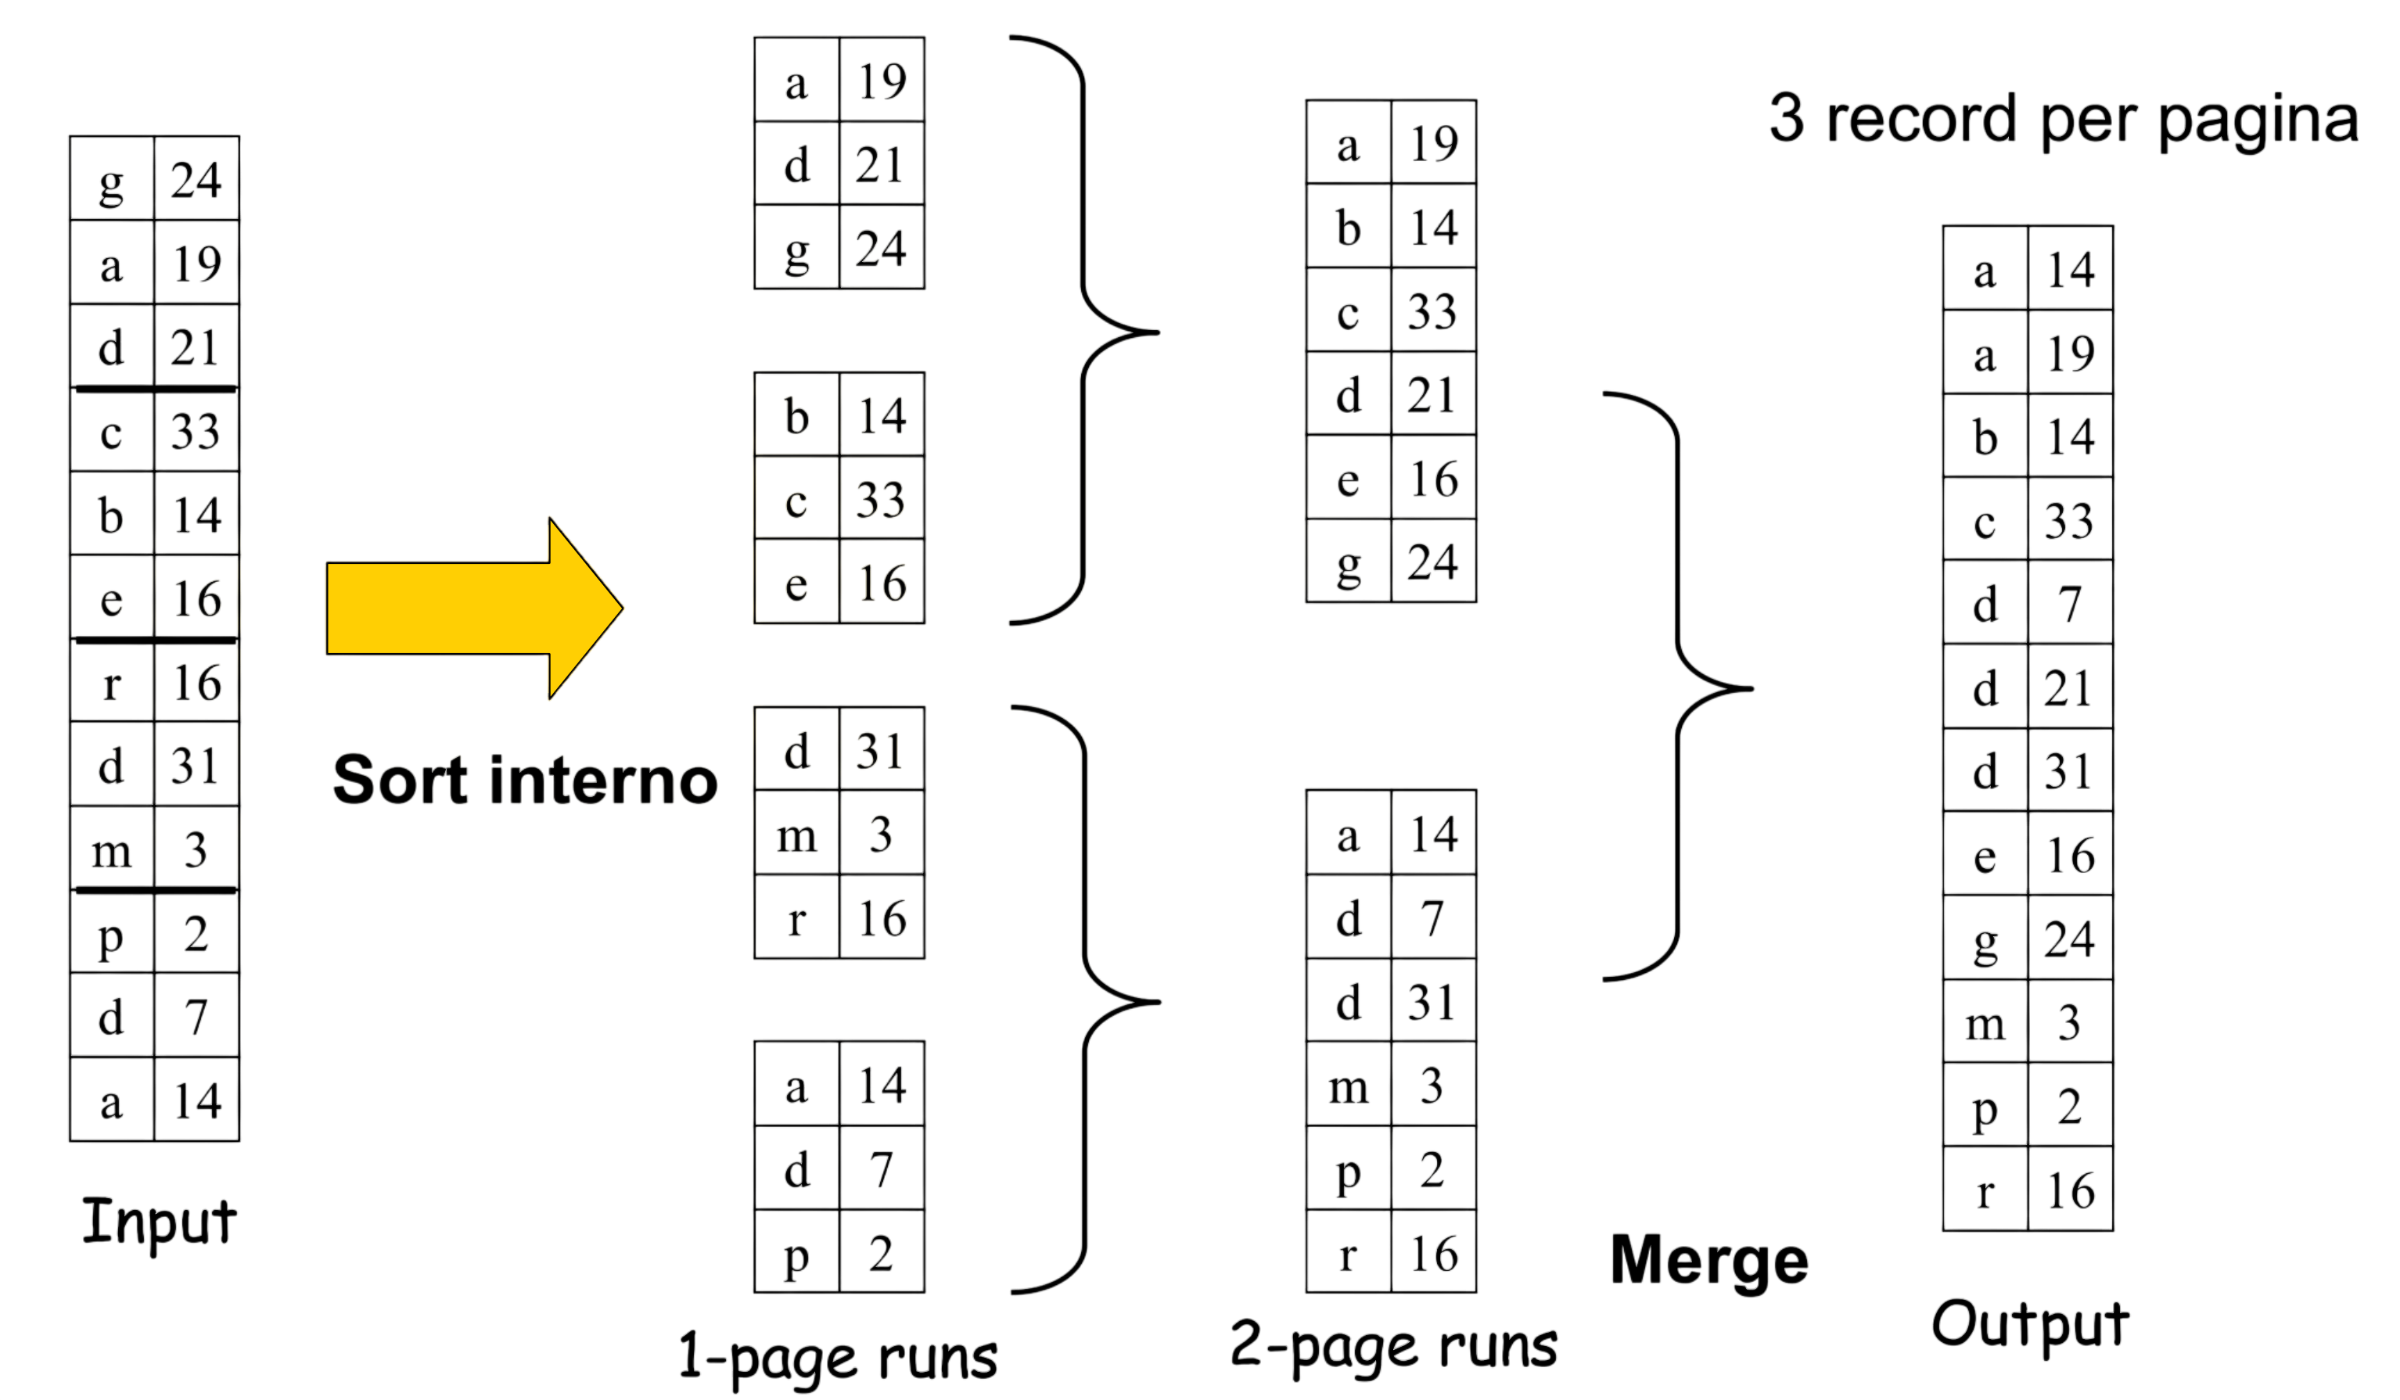
\includegraphics[width=0.6\textwidth]{images/ordinamento-Z-way-Sort-Merge.png}
    \end{figure}

    Durante il sort interno si carica e ordina una pagina alla volta ottenendo delle run ordinate.

    Si ottengono 4 run ordinate che passano alla fase di merge a due vie ($\mathrm{Z} = 2$) e si ottengono 2 run ordinate che passano ad un'ulteriore fase di merge, ottenendo così un'unica run ordinata.

    Con $\mathrm{NB} = 3$ si hanno solamente 3 buffer a disposizione, quindi, si associano 2 buffer alla run da passare alla fase di merge e 1 buffer per l'output.

    Si legge la prima pagina da ciascuna run e si genera la prima pagina dell'output, quando tutti i record di una pagina di run sono stati consumati, si legge un'altra pagina della run:
    \begin{figure}[H]
        \centering
        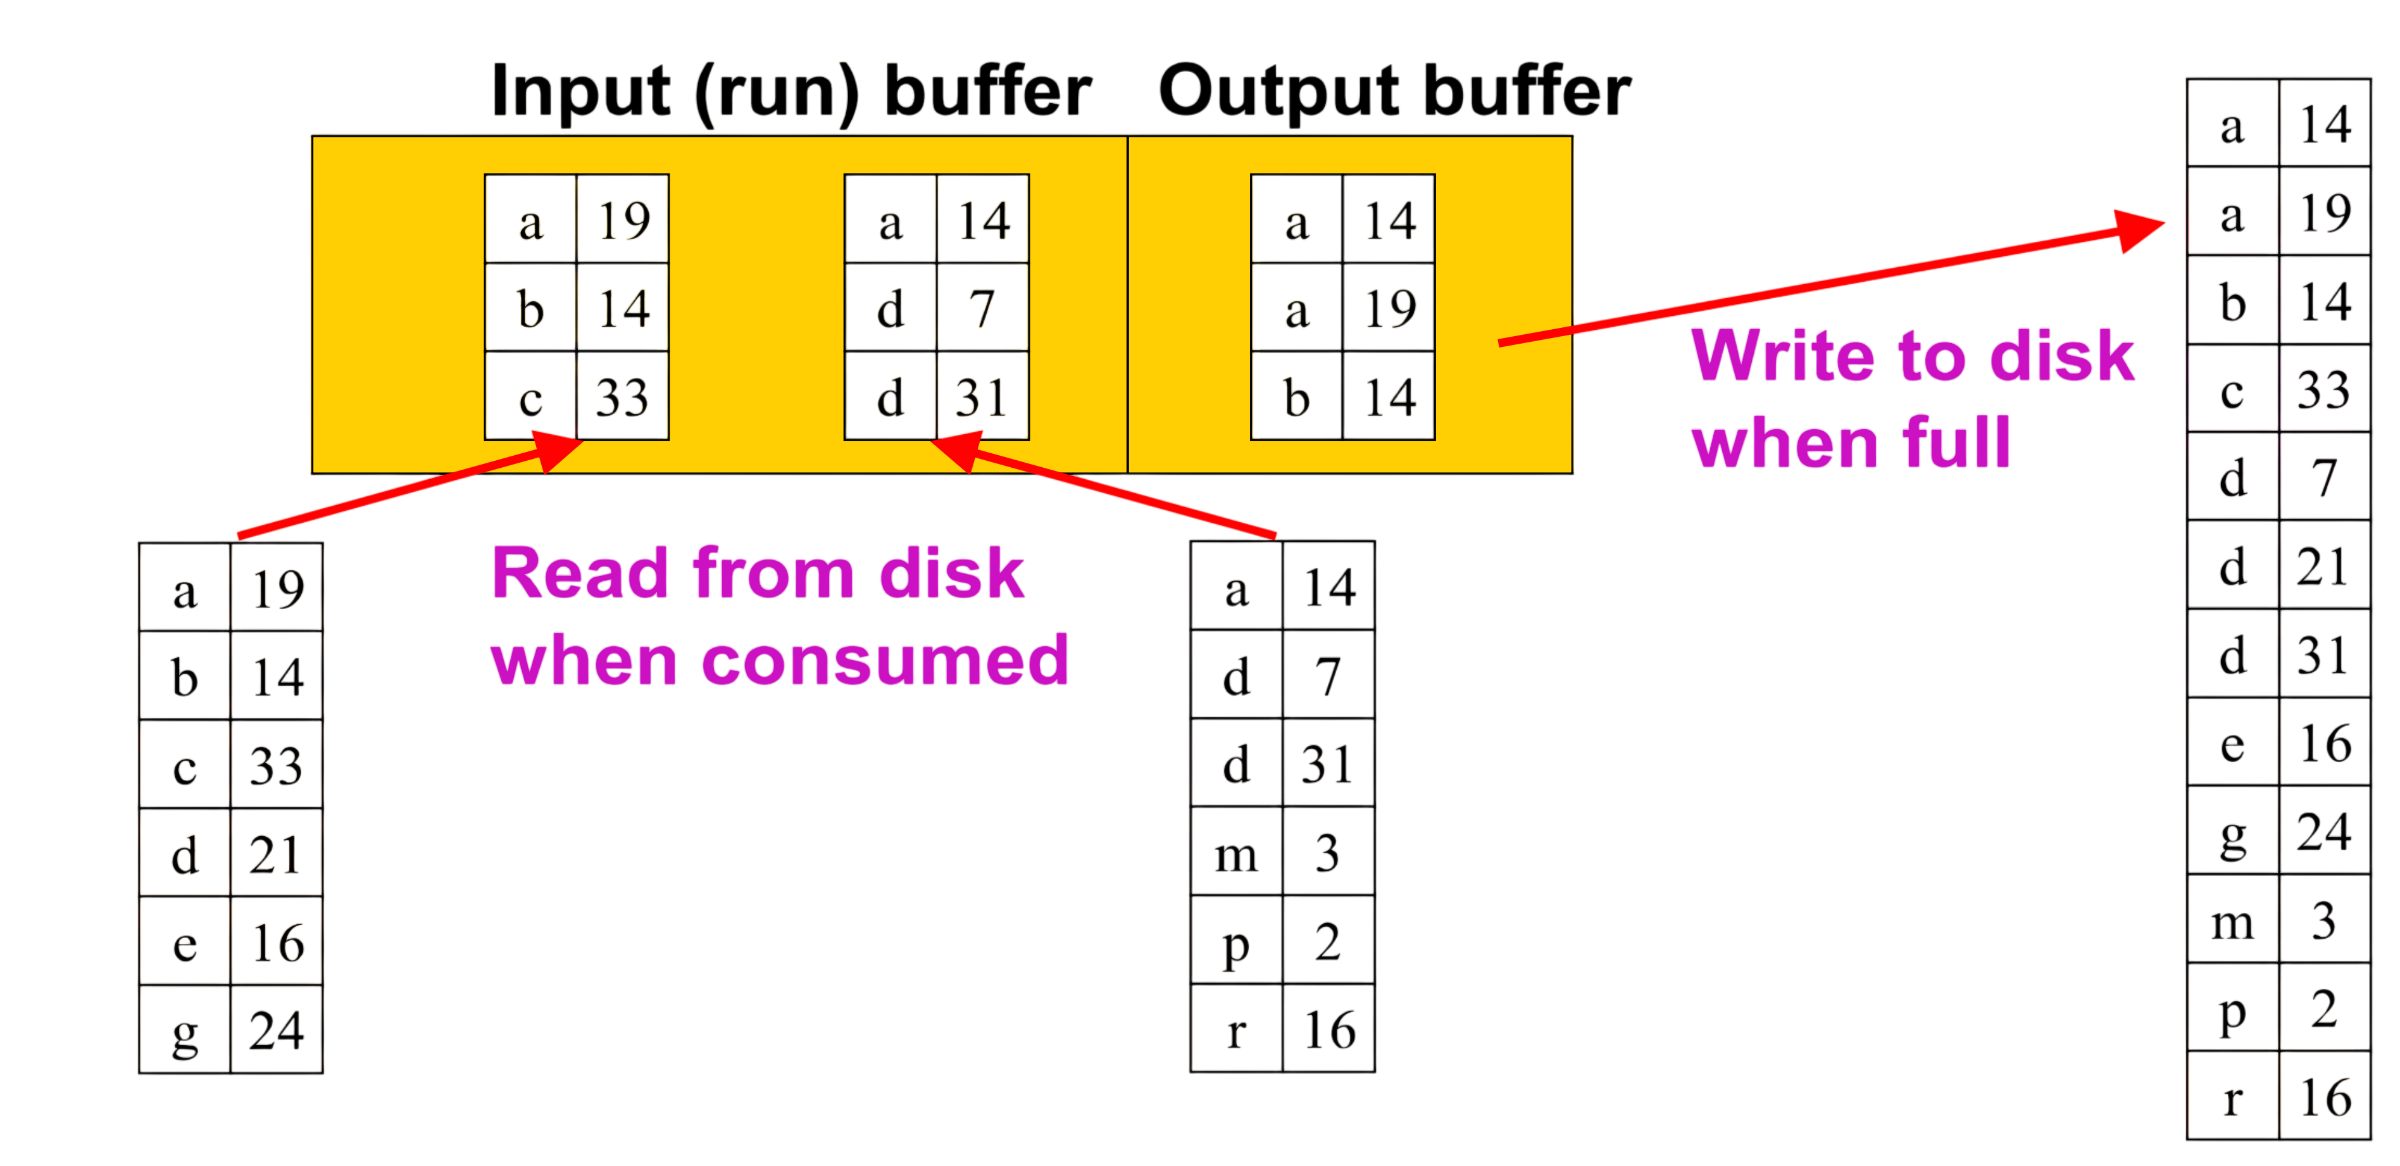
\includegraphics[width=0.6\textwidth]{images/utilizzoBuffer-Z-way-Sort-Merge.png}
    \end{figure}
}

\begin{itemize}[label=$\Rightarrow$, itemsep=\smallskipamount]
    \item \textcolor{red}{\textbf{costo ordinamento}} (con $\mathrm{Z} = 2$ e $\mathrm{NB} = 3$):
    \begin{itemize}[label=$\diamond$, itemsep=\smallskipamount]
        \item fase di sort interno: si leggono $\mathrm{NP(R)}$ pagine e si scrivono $\mathrm{NP(R)}$ pagine
        \[
            \mathrm{2 \cdot NP(R)}
        \]
        \item fase di merge: si leggono $\mathrm{NP(R)}$ pagine e si scrivono $\mathrm{NP(R)}$ pagine:
        \[
            \mathrm{2 \cdot NP(R)}
        \]
    \end{itemize}
    Il numero di passi di merge è:
    \[
        \mathrm{\lceil \log_2(NP(R)) \rceil}
    \]

    Il costo complessivo è:
    \[
        \mathbf{2 \times NP(R) \times (\lceil \log_2(NP(R)) \rceil)}
    \]
\end{itemize}

\subsection{Accesso diretto tramite indice}
Le interrogazioni che fanno uso dell'indice sono:
\begin{itemize}[label=$\diamond$, itemsep=\smallskipamount]
    \item \textbf{selezioni con condizione atomica di ugualianza} ($\mathrm{A = v}$): richiede indici di hash o B+ tree
    \item \textbf{selezione con condizione di range} ($\mathrm{A \geq v_1 \land A \leq v_2}$): richiede indice B+ tree
    \item \textbf{selezione con condizione costituita da una congiunzione di condizioni di ugualianza} ($\mathrm{A = v_1 \land B = v_2}$): l'indice viene scelto in base alla condizione più selettiva, l'altra condizione viene verificata filtrando i record restituiti dall'indice
    \item \textbf{selezioni con condizione costituita da una disgiunzione di condizioni di uguaglianza} ($\mathrm{A = v_1 \lor A = v_2}$): gli indici possono essere usati in parallelo e poi fare un merge o unione dei risultati
\end{itemize}

\subsection{Join}
Il join è l'operazione più costosa da eseguire, quindi, l'ottimizzatore è particolarmente attento ad ottimizzare questa operazione, tanto da prevedere diversi algoritmi:
\begin{itemize}[label=$\triangleright$, itemsep=\smallskipamount]
    \item \textbf{nested loop join}
    \item \textbf{merge scan join}
    \item \textbf{hash-based join}
\end{itemize}

Dal punto di vista logico il join è commutativo, ma dal punto di vista fisico c'è una differnza sostanziale tra $\mathbf{A \bowtie B}$ e $\mathbf{B \bowtie A}$ che cambia le prestazioni.

\subsubsection{Nested loop join}
Date 2 relazioni in input $\mathrm{R}$ e $\mathrm{S}$ tra cui è definito il predicato di join $\mathrm{PJ}$, distinguiamo:
\begin{itemize}[label=$\circ$, itemsep=\smallskipamount]
    \item \textbf{relazione esterna} $\mathbf{R}$
    \item \textbf{relazione interna} $\mathbf{S}$
\end{itemize}

L'algoritmo funziona come segue:
\begin{codiceSQL}
$\forall$ tupla $\mathrm{t_R}$ { --relazione esterna
    $\forall$ tupla $\mathrm{t_S}$ { --relazione interna
        if ($\mathrm{t_R, t_S}$) soddisfa PJ
            aggiungi ($\mathrm{t_R, t_S}$) al risultato
    }
}
\end{codiceSQL}

\esempio{algoritmo nested loop join}{
    Consideriamo il seguente esempio di join tra le relazioni $\mathrm{R}$ e $\mathrm{S}$:
    \begin{figure}[H]
        \centering
        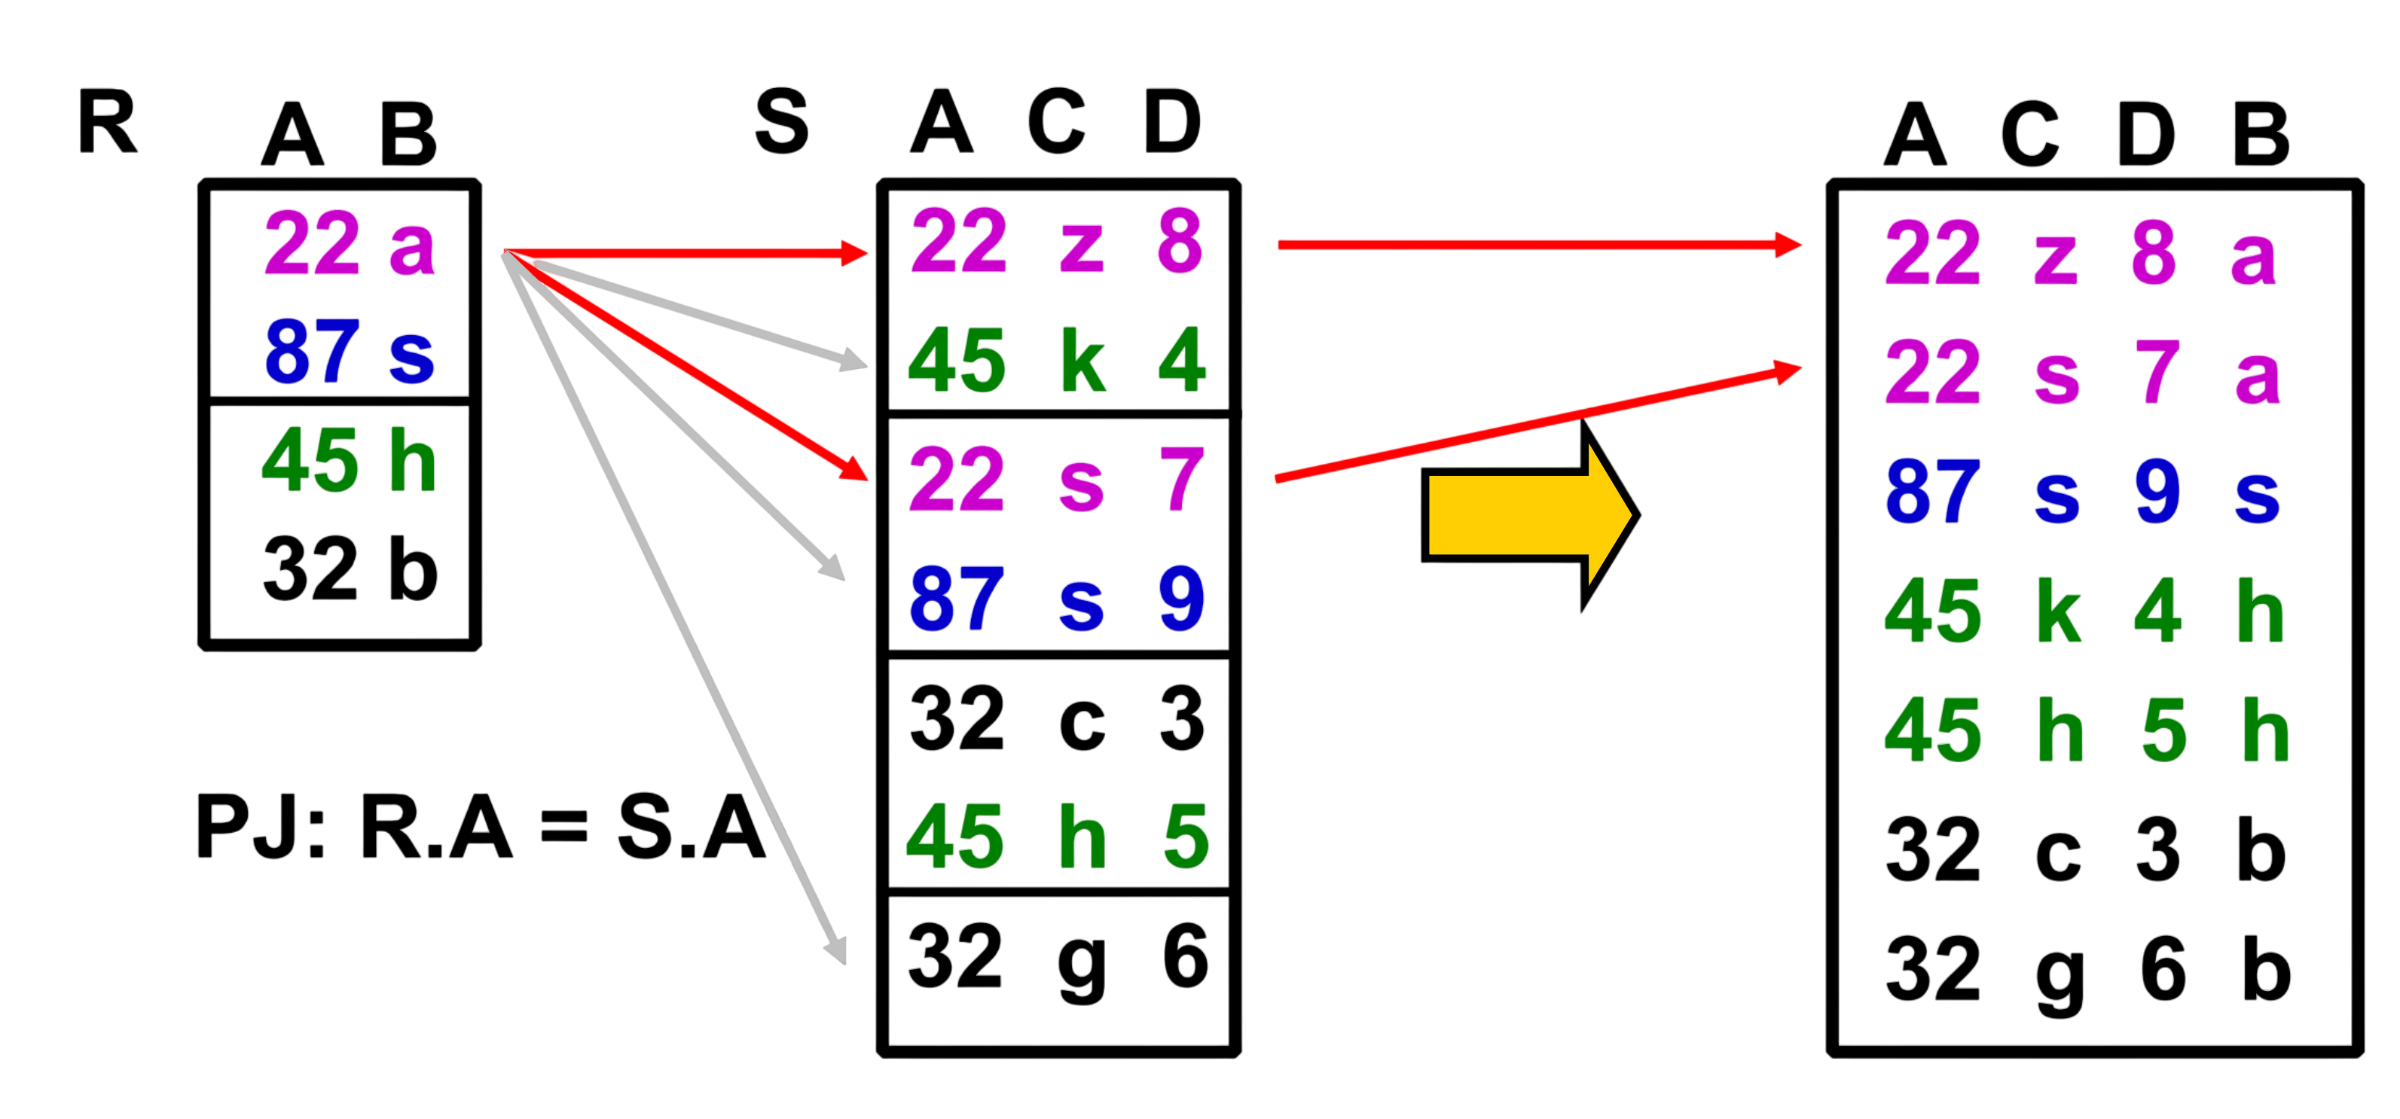
\includegraphics[width=0.5\textwidth]{images/nested-loop-join.png}
    \end{figure}

    $\mathrm{R}$ deve verificare per ogni riga di $\mathrm{S}$ che il predicato sia verificato.
}

\begin{itemize}[label=$\Rightarrow$, itemsep=\smallskipamount]
    \item \textcolor{red}{\textbf{costo nested loop join}} (consideriamo 1 pagina per caricare R e 1 pagina per caricare S):
    \begin{itemize}[label=$\diamond$, itemsep=\smallskipamount]
        \item bisogna leggere $\mathrm{R}$ completamente una volta
        \item per ogni riga di $\mathrm{R}$ ($\mathrm{NP(R) = \# \text{RIGHE R}}$) bisgona leggere completamente $\mathrm{S}$
    \end{itemize}

    \smallskip
    Il costo complessivo è:
    \[
        \mathbf{NP(R) + NR(R) \cdot NP(S)}
    \]
\end{itemize}

A seconda del numero di righe di $\mathrm{R}$ cambia il numero di volte che bisogna leggere $\mathrm{NP(R)}$, quindi, la relazione esterna deve essere quella più piccola per minimizzare il costo.

\subsubsection{Nested loop join con indice}
Data una relazione esterna $\mathrm{R}$ e una interna $\mathrm{S}$, si ha che la scansione completa di $\mathrm{S}$ può essere sostituita dalla scansione basata sull'indice costituito sugli attributi di join di $\mathrm{S}$.

\esempio{algoritmo nested loop join con indice}{
    Consieriamo il seguente esempio di nested loop join con indice tra le relazioni $\mathrm{R}$ e $\mathrm{S}$:
    \begin{figure}[H]
        \centering
        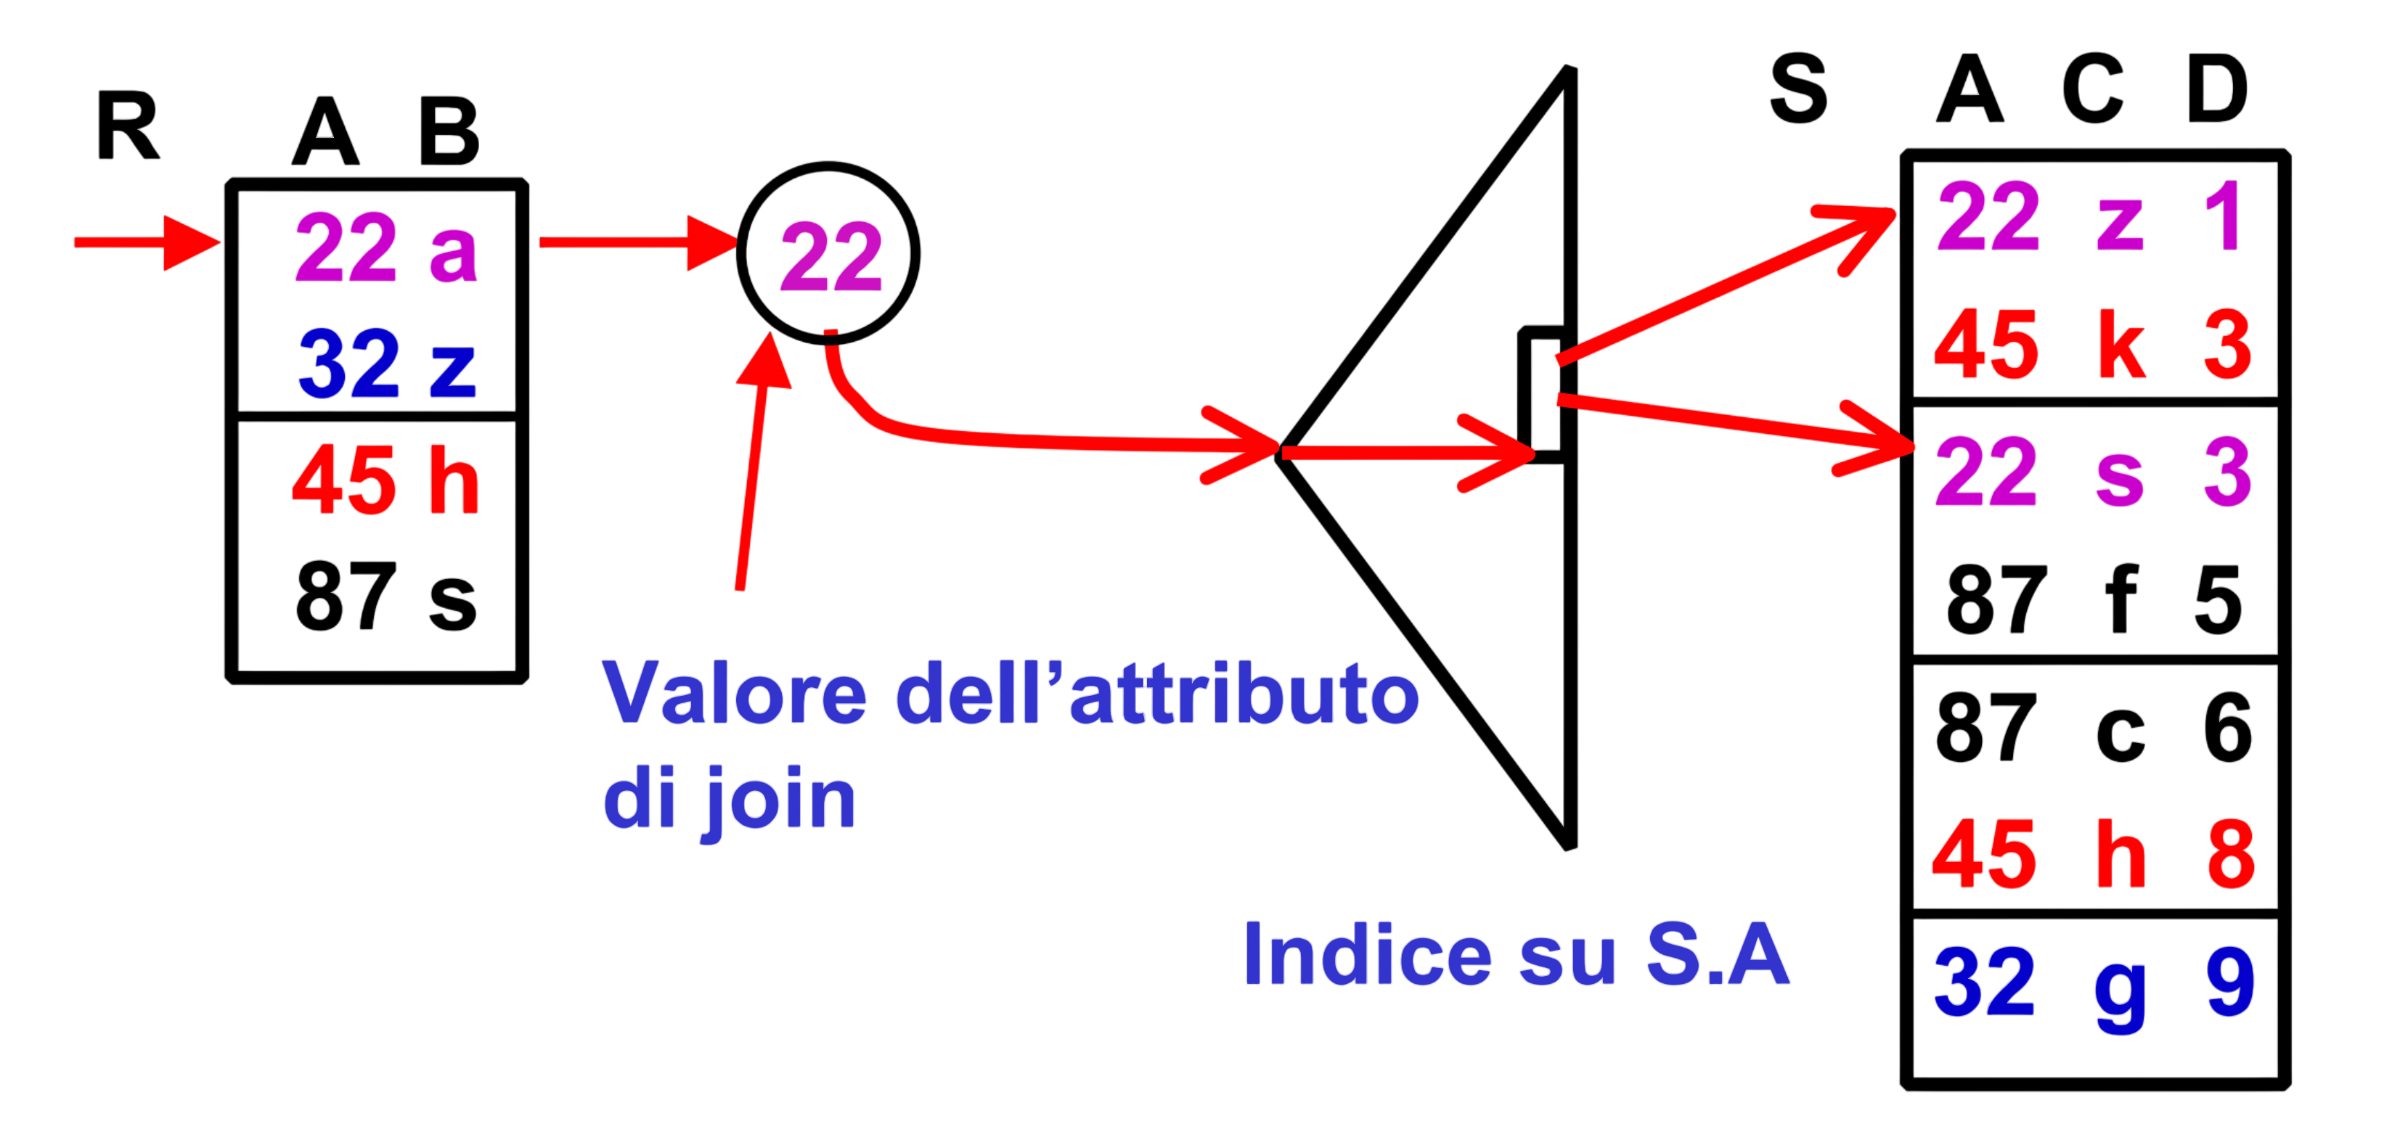
\includegraphics[width=0.5\textwidth]{images/nested-loop-join-indice.png}
    \end{figure}

    L'indice su $\mathrm{S.A}$ permette di caricare solo i blocchi di $\mathrm{S}$ che contengono l'attributo $\mathrm{A = 22}$.
}

\begin{itemize}[label=$\Rightarrow$, itemsep=\smallskipamount]
    \item \textcolor{red}{\textbf{costo nested loop join}} (usando B+ tree):
    \[
        \mathbf{NP(R) + NR(R)} \cdot \left(\text{ProfonditàIndice} + \mathbf{\frac{NR(S)}{VAL(A,S)}}\right)
    \]
\end{itemize}

La tabella $\mathrm{R}$ deve comunque essere caricata tutta ($\mathrm{NP(R)}$) e rimane invariato anche il numero di volte che si esegue il ciclo esterno ($\mathrm{NR(R)}$).\\[0.2ex]
Ciò che cambia è il numero di blocchi/pagine di $\mathrm{S}$ che si devono caricare tutte le pagine di ($\left(\text{ProfonditàIndice} + \mathrm{\frac{NR(S)}{VAL(A,S)}}\right)$).\\[0.2ex]
L'idea è, invece, di caricare tutte le pagine di $\mathrm{S}$ si caricano solo quelle che contengono $\mathrm{S.A = R.A}$
\begin{itemize}[label=$\diamond$, itemsep=\smallskipamount]
    \item $\mathbf{\frac{NR(S)}{VAL(A,S)}}$: rappresenta la stima di quanti blocchi di $\mathrm{S}$ contengono $\mathrm{A}$ uguale al valore interessato.
    
    Questa stima è anche chiamata \textbf{selettività} dell'attributo $\mathrm{A}$.
    \item $\mathbf{VAL(A,S)}$: numero di valori distinti di $\mathrm{A}$ che compaiono in $\mathrm{S}$
\end{itemize}

\esempio{}{
    Supponiamo che $\mathrm{A} = \text{Nome\_Regioni}$, quindi, il numero di possibili valori di $\mathrm{A}$ è 21.

    Consideriamo:
    \begin{itemize}[label=$\diamond$, itemsep=\smallskipamount]
        \item $\mathrm{NR(S) = 2100}$
        \item numero di righe per ogni regione è:
        \[
            \mathrm{\frac{NR(S)}{VAL(A,S)} = \frac{2100}{21} = 1000}
        \]

        quindi si ha l'assunzione che il dato sia unififorme, cioè che non siano più o meno lo stesso numero di pagine per ogni regione
        \item nel caso pessimo si ha un blocco/pagina per ogni riga
    \end{itemize}

    \smallskip
    Quindi, il costo del nested loop join con indice è:
    \[
        \begin{aligned}
            &\mathbf{NP(R) + NR(R)} \cdot \left(\text{ProfonditàIndice} + \mathbf{\frac{NR(S)}{VAL(A,S)}}\right)\\
            &\mathbf{NP(R) + NR(R) \cdot (\text{ProfonditàIndice} + 1000)}
        \end{aligned}
    \]
}

\subsubsection{Block nested loop join}
Il \textbf{block nested loop join} è una variante del nested loop in cui ciascuna pagina di $\mathrm{S}$ (tabella interna) viene letta per ogni pagina di $\mathrm{R}$ (tabella esterna), invece, che per ogni riga di $\mathrm{R}$.\\[0.2ex]
Lo pseudocodice è il seguente:
\begin{codiceSQL}
$\forall$ pagina $\mathrm{P_R}$ di R { --relazione esterna
    $\forall$ pagina $\mathrm{P_S}$ di S { --relazione interna
        $\forall$ tupla $\mathrm{t_R}$ di $\mathrm{P_R}$ {
            $\forall$ tupla $\mathrm{t_S}$ in $\mathrm{P_S}$ {
                if ($\mathrm{t_R}$ , $\mathrm{t_S}$) soddisfa PJ
                    aggiungi ($\mathrm{t_R}$ , $\mathrm{t_S}$) al risultato
            }
        }
    }
}
\end{codiceSQL}

\begin{itemize}[label=$\Rightarrow$, itemsep=\smallskipamount]
    \item \textcolor{red}{\textbf{costo block nested loop join}}: dipende dallo spazio a disposizione nei buffer.
    
    Supponiamo di avere 1 buffer per R e 1 buffer per S, allora:
    \begin{itemize}[label=$\diamond$, itemsep=\smallskipamount]
        \item bisogna leggere R completamente una volta, quindi NP(R)
        \item per ogni pagina di R (NP(R)) bisogna leggere completamente S quindi NP(R) NP(S)
    \end{itemize}

    \smallskip
    Il costo totale è:
    \[
        \mathbf{NP(R) + NR(R) \cdot NP(S)}
    \]
\end{itemize}

\esempio{algoritmo block nested loop join}{
    Consideriamo il seguente esempio di block nested loop join tra le relazioni R e S:
    \begin{figure}[H]
        \centering
        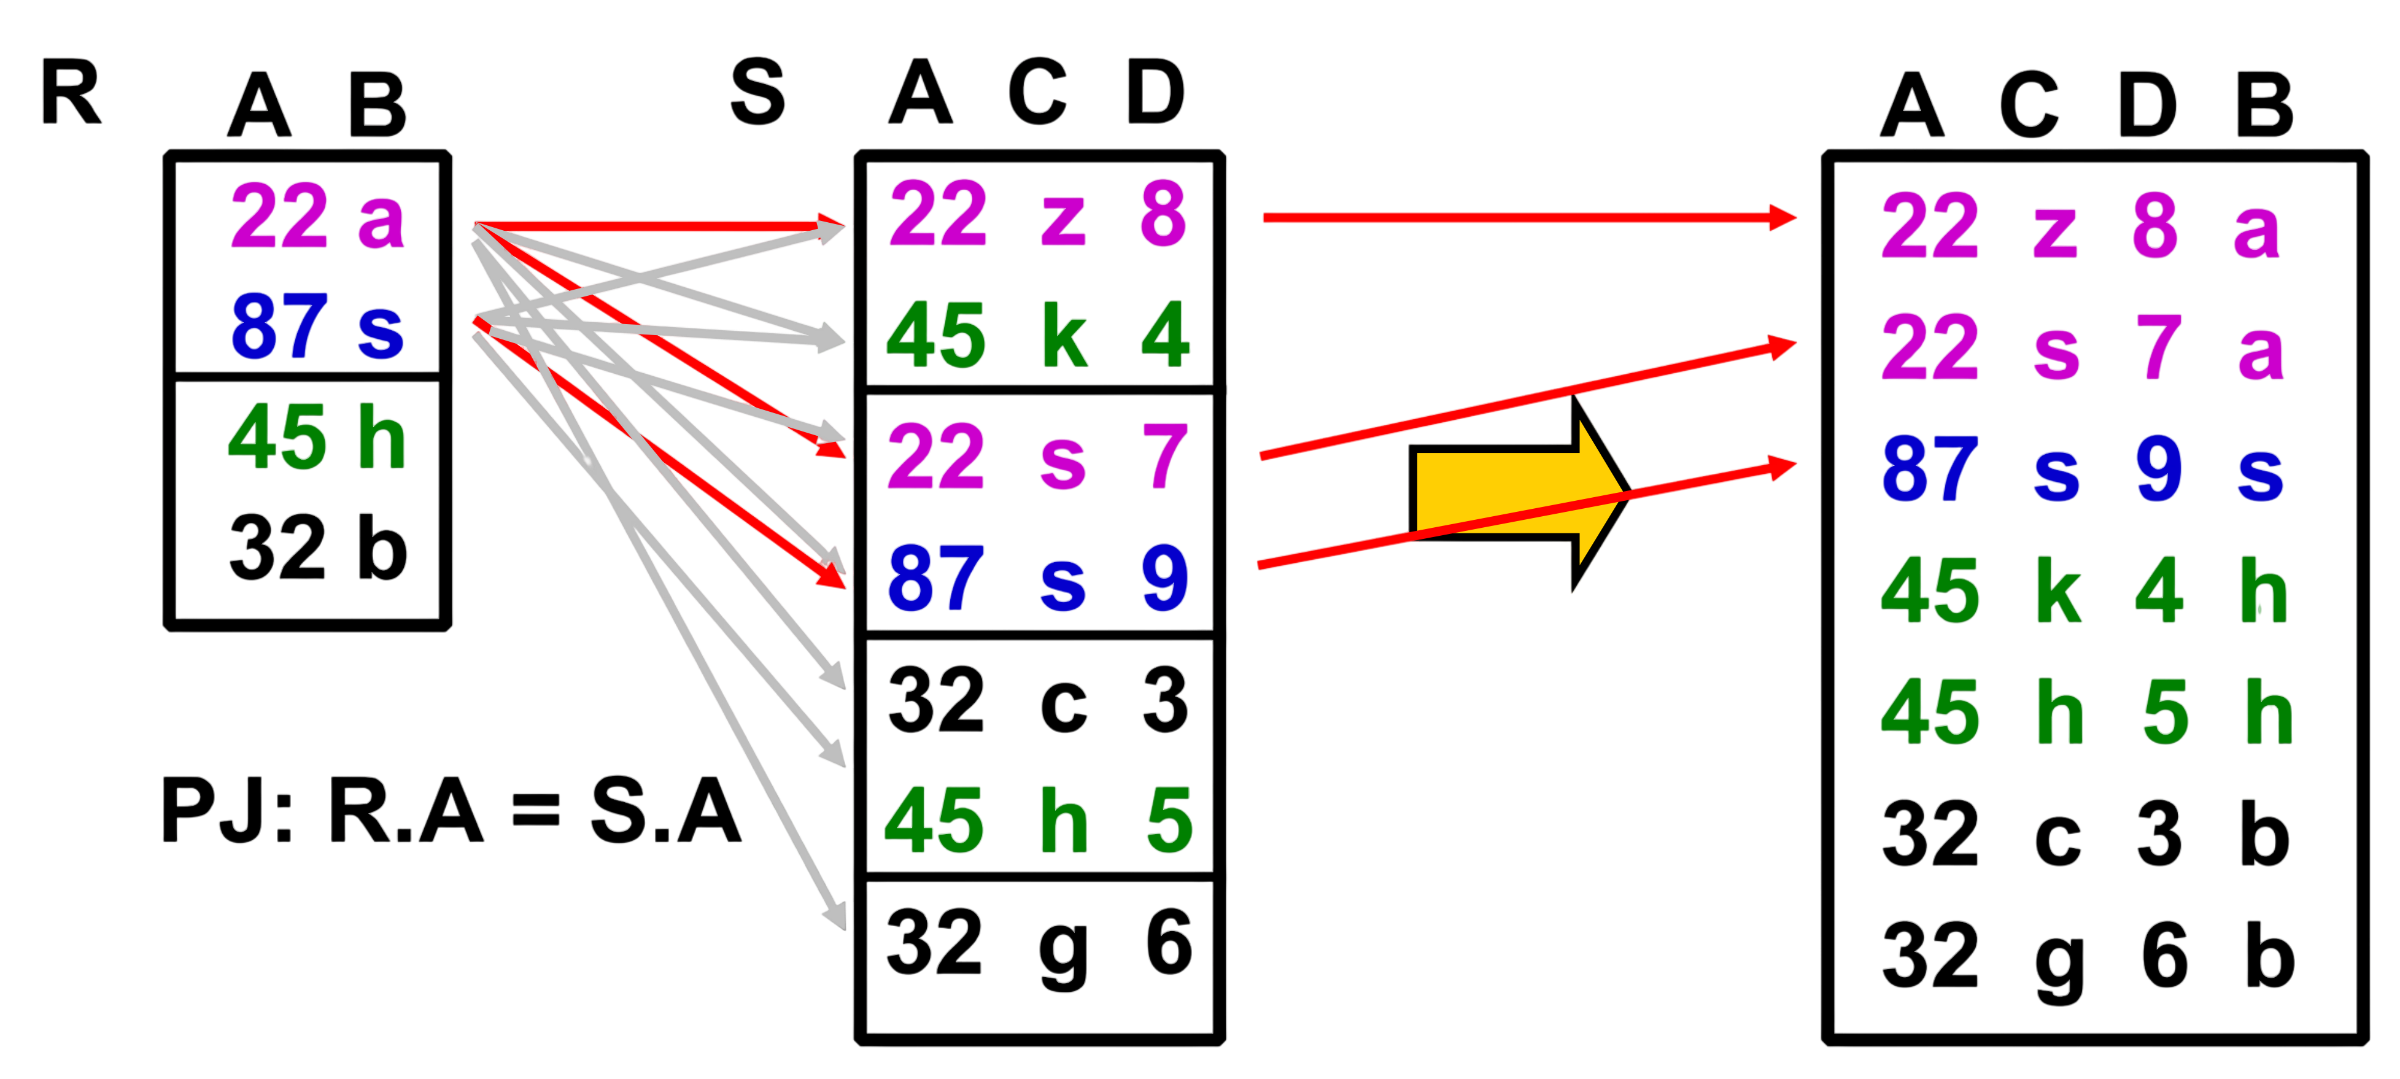
\includegraphics[width=0.5\textwidth]{images/block-nested-looop-join.png}
    \end{figure}
}

\subsubsection{Merge scan join}
Il \textbf{merge scan join} è applicabile quando entrambi gli insiemi di tuple in input sono ordinati sugli attributi di join e il join è un equi-join (predicato di join è una condizone di uguaglianza).\\[0.2ex]
Cià accade sia per entrambe le relazioni $\mathrm{R}$ e $\mathrm{S}$ vale almeno una delle seguenti condizioni:
\begin{itemize}[label=$\circ$, itemsep=\smallskipamount]
    \item relazione è fisicamente ordinata sugli attributi di join (file sequenziale ordinato come struttura fisica)
    \item esiste un indice sugli attributi di join della tabella che consente una scansione ordinata delle tuple
\end{itemize}

La logica di questo algoritmo sfrutta il fatto che entrambi gli input sono ordinati per evitare di fare confronti inutili e questo fa si che il numero di letture totali sia:
\[
    \mathbf{NP(R) + NP(S)}
\]

se si accede sequenzialmente alle due relazioni ordinate fisicamente.

\begin{itemize}[label=$\circ$, itemsep=\smallskipamount]
    \item con indici B+ tree su entrambe relazioni i costo può arrivare al massimo (con indici nel buffer) a:
    \[
        \mathbf{NR(R) + NR(S)}
    \]
    \item con una relazione ordinata e un solo indice il costo è al massimo:
    \[
        \mathbf{NP(R) + NR(S)} (\text{o viceversa})
    \]
\end{itemize}

\esempio{algoritmo merge scan join}{
    Consideriamo il seguente esempio di merge scan join tra le relazioni $\mathrm{R}$ e $\mathrm{S}$:
    \begin{figure}[H]
        \centering
        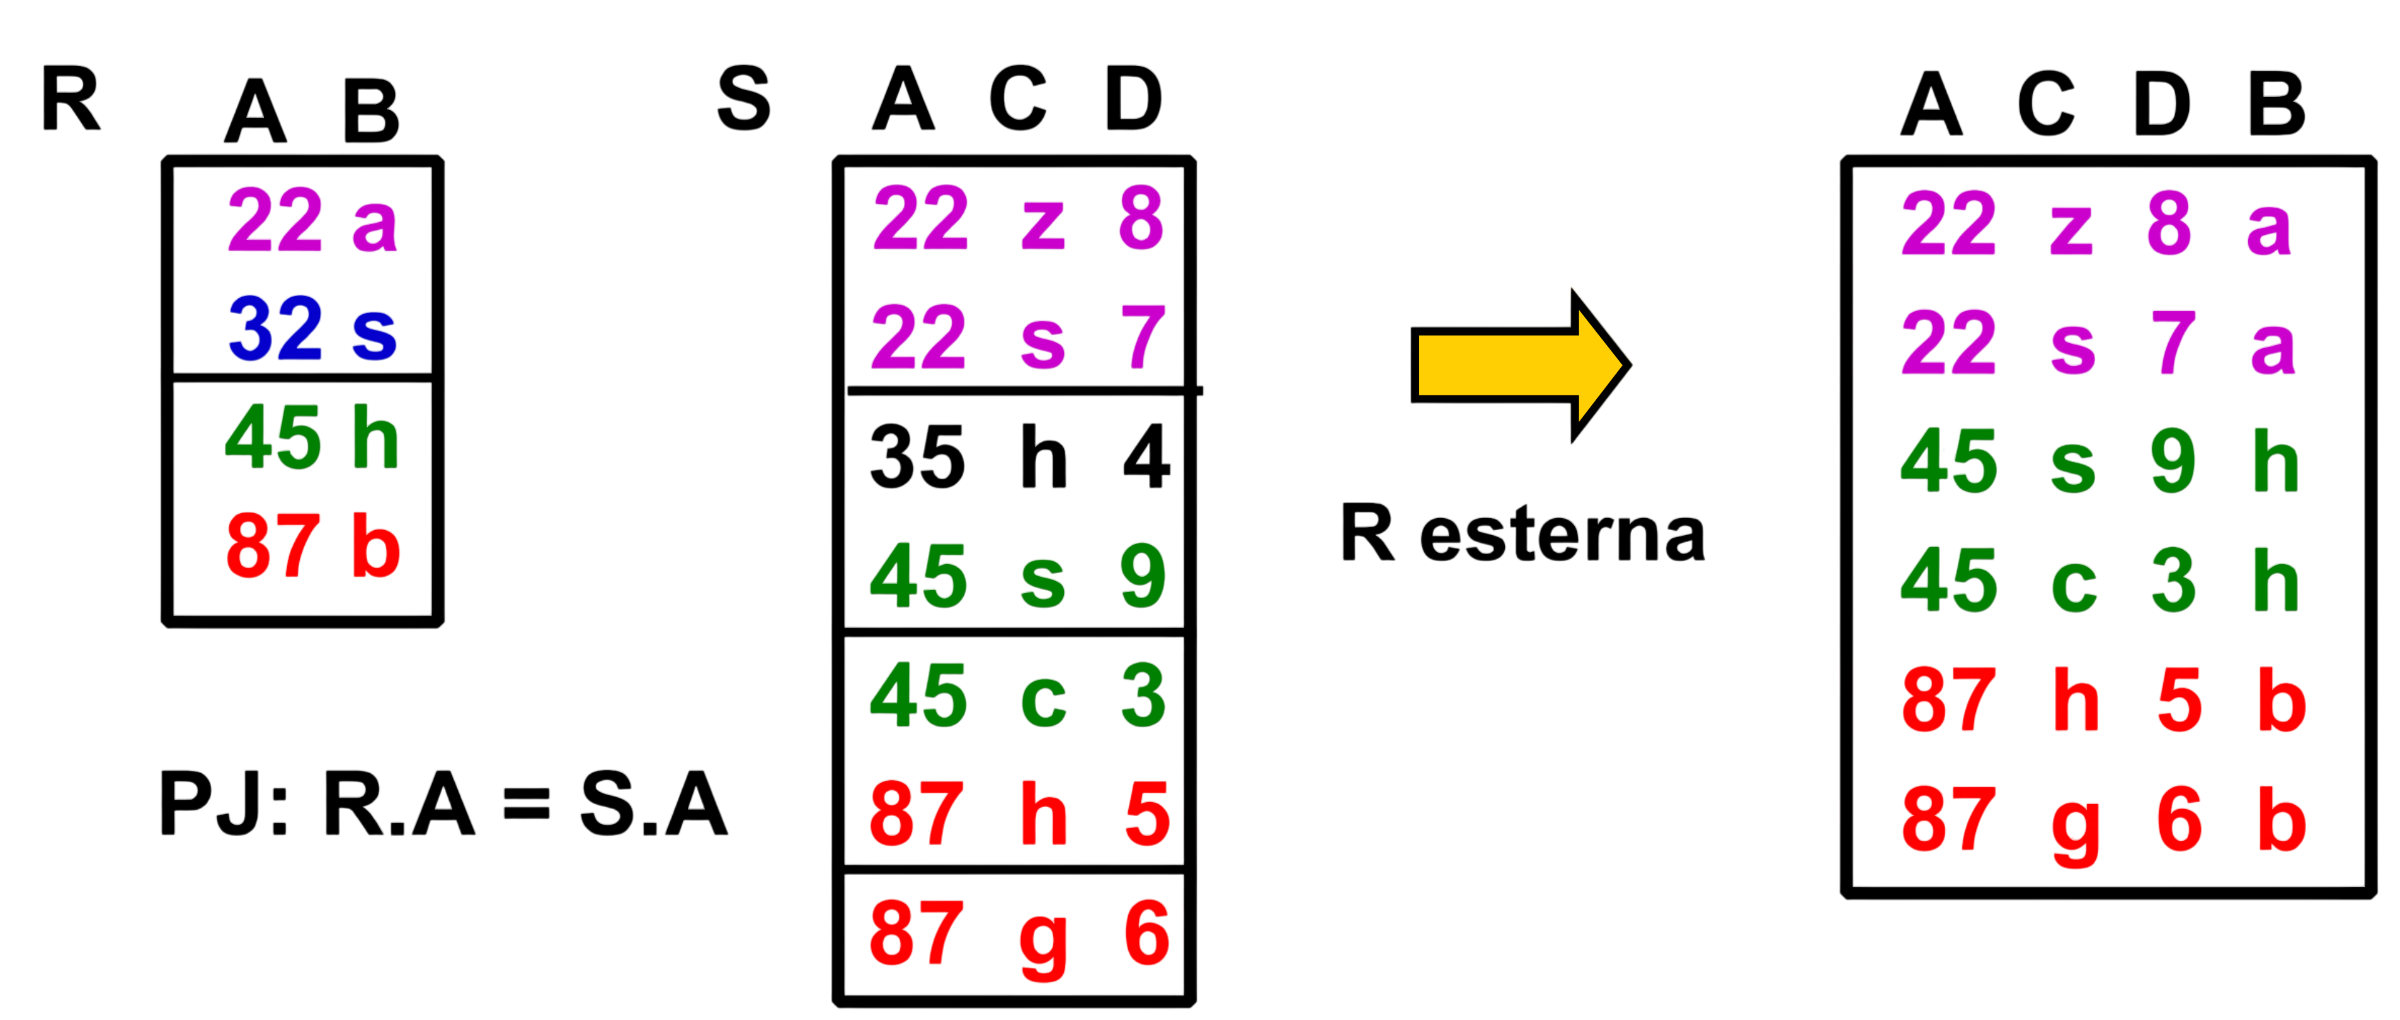
\includegraphics[width=0.5\textwidth]{images/merge-scan-join.png}
    \end{figure}
}

\subsubsection{Hash-based join}
L'algoritmo di \textbf{hash-based join} è applicabile solo in caso di equi-join e non richiede nè la presenza di indici nè input ordinati e risulta particolarmente vataggioso in caso di relazioni molto grandi.\\[0.2ex]
L'idea sui cui si basa l'hash join è semplice: si suppone di avere a disposizione una funzione hash $\mathrm{h}$ che viene applictaa agli attributi di join delle due relazioni (es. $\mathrm{R.J}$ e $\mathrm{S.J}$).

\begin{itemize}[label=$\circ$, itemsep=\smallskipamount]
    \item se $\mathrm{t_R}$ e $\mathrm{t_S}$ sono 2 tuple di $\mathrm{R}$ e $\mathrm{S}$, allora è possibile che sia $\mathrm{tR.J = tS.J}$ solo se $\mathrm{h(tR.J) = h(tS.J)}$
    \item se, viceversa, $\mathrm{h(tR.J) \neq h(tR.J)}$, allora si ha $\mathrm{tR.J \neq tS.J}$
\end{itemize}

Da questa idea si hanno diverse implementazioni, che hanno in comune il fatto che $\mathrm{R}$ e $\mathrm{S}$ vengono partizionate sulla base dei valori della funzione di hash $\mathrm{h}$, e che la ricerca di matching tuples aviene solo tra partizioni relative allo stesso valore di $\mathrm{h}$.

$\Rightarrow$ \textcolor{red}{\textbf{costo hash-based join}}:
\begin{itemize}[label=$\circ$, itemsep=\smallskipamount]
    \item costruzione dell'hash map:
    \[
        \mathbf{NP(R) + NP(S)}
    \]
    \item accesso alle matching tules che nel caso pessimo può costare:
    \[
       \mathbf{ NP(R) \cdot NP(S)}
    \]
\end{itemize}

\section{Scelta del piano esecuzione}
Data un'espressione ottimizzata in algebra, i passi da eseguire sono:
\begin{enumerate}[itemsep=\smallskipamount]
    \item \textbf{si generano tutti i possibili paini di esecuzione} (alberi) \textbf{alternativi} (o un sottoinsieme) \textbf{ottenuti considernando le seguenti dimensioni}
    \begin{itemize}[label=$\circ$, itemsep=\smallskipamount]
        \item operatori alternativi applicabili per l'accesso ai dati: scan sequenziale o via indice
        \item operatori alternativi applicabili nei nodi: nested loop join o hash based join
        \item ordine delle operazioni da compiere (associatività)
    \end{itemize}
    \item \textbf{si valuta con formule approssimate il costo di ogni alternativa in termini di accessi alla memoria secondaria richiesti} (è una stima)
    \item \textbf{si sceglie l'albero con il costo stimato minimo}
\end{enumerate}

Nella valutazione delle stime di costo si tiene conto del profilo delle relazioni, solitamente memorizzato nel data directory e contente per ogni relazione $\mathrm{T}$:
\begin{itemize}[label=$\circ$, itemsep=\smallskipamount]
    \item stima della cardinailtà (\# tuple): $\mathrm{CARD(T)}$
    \item stima della dimensione di una tupla: $\mathrm{SIZE(T)}$
    \item stima della dimensione di ciascun attributo $\mathrm{A}$: $\mathrm{VAL(A,T)}$
    \item stima del numero di valori distinti per ogni attributo $\mathrm{A}$: $\mathrm{MAX(A,T)}$ e $\mathrm{MIN(A,T)}$
\end{itemize}

\begin{esempiobox}{Esercizio}
    Consideriamo la seguente base di dati:
    \[
        \begin{aligned}
            &\texttt{INGREDIENTE(\underline{codice}, nome, calorie)}\\
            &\texttt{COMPOSIZIONE(\underline{ricetta, ingrediente}, quantità)}\\
            &\texttt{RICETTA(\underline{codiceRicetta}, nome, regione, tempoPreparazione)}
        \end{aligned}
    \]

    e i seguenti vincoli d'integrità:
    \[
        \begin{aligned}
            &\text{Composizione.ricetta} \rightarrow \text{Ricetta}\\
            &\text{Composizione.ingrediente} \rightarrow \text{Ingrediente}
        \end{aligned}
    \]

    Data la seguente query:
\begin{codiceSQL}
SELECT R.codiceRicetta, I.nome, I.calorie
FROM RICETTA R
JOIN Composizione C ON R.codiceRicetta = C.ricetta
JOIN Ingrediente I ON C.Ingrediente = I.codice
    WHERE R.regione = 'Veneto';
\end{codiceSQL}

    \textcolor{red}{\textbf{Calcolare il costo dell'interrogazione in termini di numero di accessi alla memoria sedcondaria con le seguenti ipotesi:}}
    \begin{itemize}[label=$\circ$, itemsep=\smallskipamount]
        \item la selezione (\texttt{R.Veneto = 'Veneto'}) su \texttt{Riccetta} richiede una scansione sequenziale della tabelle \texttt{Ricetta}.
        
        Inoltre, la selezione rimane nel buffer.
        \item l'ordine di esecuzione del join è:
        \[
            (\text{Ricetta} \Join \text{Composizione}) \Join \text{Ingrediente}
        \]
        \item le operazioni di join vengono eseguite con la tecnica nested loop join con 1 pagina di buffer a disposizione per ogni tabella
        \item il risultato del primo join ($\text{Ricetta} \Join \text{Composizione}$) viene interamente mantenuto nel buffere
        \item il numero di pagine e righe per ogni tabella è il seguente:
        \begin{table}[H]
            \centering
            \begin{tabular}{|c|c|c|c|c|c|}
                \hline
                Tabella & NP & NR & VAL(regione) & VAL(Ricetta) & VAL(Qtà)\\
                \hline
                Ingrediente & 30 & 270 & & & \\
                Composizione & 780 & 19800 & & 90 & 50\\
                Ricetta & 150 & 900 & 18 & \\
                \hline
            \end{tabular}
        \end{table}
    \end{itemize}

    \textbf{Svolgimento}
    \begin{enumerate}[itemsep=\medskipamount]
        \item \textbf{selezione su ricetta}:
        \item \textbf{join su Composizione}:
        \item \textbf{join su Ingrediente}:
    \end{enumerate}
\end{esempiobox}
